% Copyright (c) 2014,2016,2018 Casper Ti. Vector
% Public domain.

\chapter{地形语义信息的生成与编辑}
地形语义是对地形高程或纹理数据在现实世界中所表示的含义和特征进行解释。虚拟现实系统在具体项目应用中常兼顾地理信息系统的功能\supercite{沈敬伟},这时往往需要地形模块以语义信息的形式描述地理环境,并提供给其他模块。为地形块挂载语义可以扩展虚拟现实系统的应用场景。\par
地形语义信息可以作为其他模块绘制的依据,如指示水域绘制的范围或者植被的分布区域。从高空中观察地形时,陆地与海洋交界生成的海岸线是一个重要的视觉特征。由于陆地由静态网格生成,海洋由动态网格生成,因此除了卫星影像上呈现出陆地与海洋颜色的分界线外,海洋网格与陆地网格在绘制深度上有远近之分,网格间相互遮挡也在视觉上构成分界线。但这样形成的海岸线视觉上看来非常不平滑、不自然,如图6.1所示。用纹理笔刷对海岸线进行描绘可以改善高空观看时海岸线的锯齿效果,但受地形高程分辨率影响,海域范围内如码头、礁石等细长物体在高空观看时依然有强烈的锯齿。为地形提供语义信息,从而为海洋网格的绘制范围提供指导是一个可行的思路。\par
\begin{figure}[H]
    \centering
    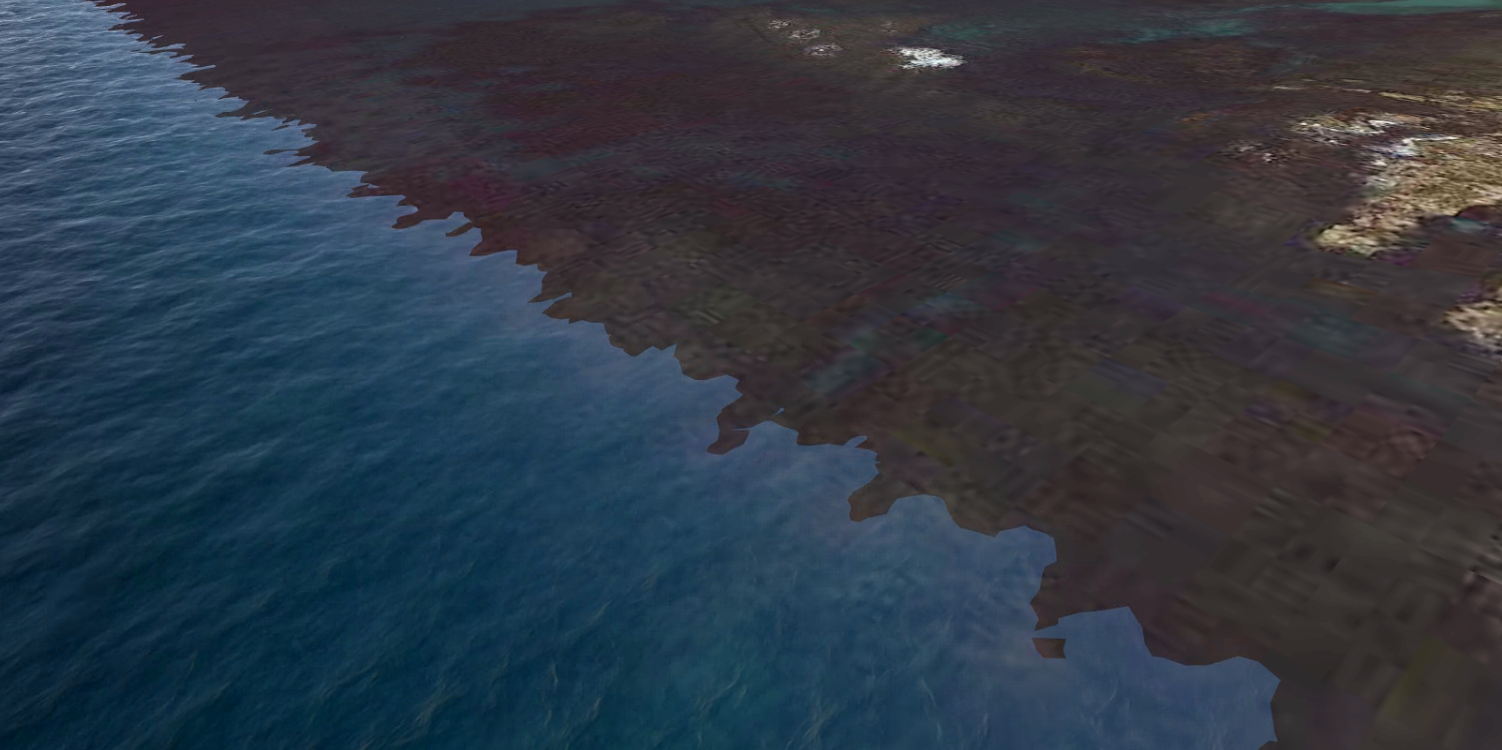
\includegraphics[height=4.4cm,width=7cm]{figures/shoreBad.png}
    \caption{陆地和海洋网格分别绘制、相互遮挡,形成的海岸线视觉效果不好}
\end{figure}
语义信息也可以为其他模块的计算提供依据,例如,无人车驱动算法验证应用中需要将地形信息提供给人工智能模块,以判断交通工具从地形上通过的可行性。此外,一些应用可能对地形有额外的标注信息,作为算法的输入。在战场模拟应用中,战场环境信息中包括对“夺控区”的预定义,载具驱动算法需要从地形模块获取“夺控区”的位置信息,以对行进路线进行规划。
\section{语义信息定义}
语义信息的定义存在一定的困难,因为地形的语义信息可以包含多个层次,且层次之间没有包含关系。就信息表达的内容上来说,这里提出一种语义的描述方式,将语义内容分为三种,分别是描述地形形状的地貌语义(如山地、丘陵、平原等)、描述地物的对象语义(如道路、建筑、机场跑道等)和描述地表材质的材质语义(如水面、草地、水泥、沙土等)。地貌语义可以为载具AI路线规划提供依据,对象语义可以为模型摆放、城市建筑生成、路网绘制等功能提供依据,材质语义可以为植被绘制、水体绘制、载具与地表间的摩擦力计算等功能提供依据。上述三个层次之间虽有所重合但不能相互包含,如道路的材质可以是水泥或沥青的,而水泥材质的有可能是道路也可能是建筑。因此将不同层次的语义进行分离可以更清晰完整的定义语义信息所表达的内容。将不同层次的语义以类似图层的方式组织。\par
在数据的粒度上,语义信息的组织有两个层次:地形块级别和像素级别,块级别语义对整个地形块的语义进行描述,像素级别语义类似高程和纹理信息的以二维点阵的方式离散的描述地形语义。在一些情境下语义信息的表达是比较稀疏的,如在大面积的连续的海洋或陆地地形上,其地貌语义很可能在整个地形块上都是相同的,这时在像素级别对语义信息进行存储和表示存在较大的冗余。对于上述的语义内容的三个层次,可以根据具体应用的需要提供相应的语义层,并分别对每个语义层提供块级别的数据或像素级别的数据。\par
\section{语义信息生成及编辑}
地形语义数据的覆盖范围与地形高程和纹理数据相同,且语义信息与高程和纹理数据有强相关性,可以根据高程或纹理数据自动生成。如,材质语义信息可以基于对地形纹理数据的图像语义识别生成,地貌语义可以基于对地形高程数据的分析生成。块级别和像素级别在单位数据上使用同样的格式进行表示,记作$semDataType$,这里用无符号字符类型作为$semDataType$,用枚举值进行填充。块级别的语义表示中,每个语义层的值由一个$semDataType$表示,像素级别的语义表示中,每个像素都有若干语义层的信息,每个层由一个$semDataType$表示。如果整块地形的某一层的语义信息内容相同,则在块级别语义中进行记录,而不为像素级语义分配内存。如果块内语义信息不统一的话则将块语义置为未知,并记录像素级语义。在保存在数据库中的语义数据块中,每个块的第一个字节标记是该块以何种级别存储语义,从数据库中读取并解析语义信息时根据这个标识决定后面的数据如何读取。\par
除了上文定义的三种语义层次,语义还可能有其他自定义表达,将具体语义内容的输出与语义生成的流程进行分离可以实现更好的扩展性。图6.2展示了一种较为灵活的语义生成框架,其中语义信息生成器和补丁数据为语义生成方法的使用者,语义生成方法的基类掌握语义数据生成的流程,并在派生类中实现根据源数据生成语义的具体方法。通过语义信息生成器,可以遍历源数据库中全部地形块,为有合法数据的地形块生成语义信息,并输出到目标数据库中。
\begin{figure}[H]
    \centering
   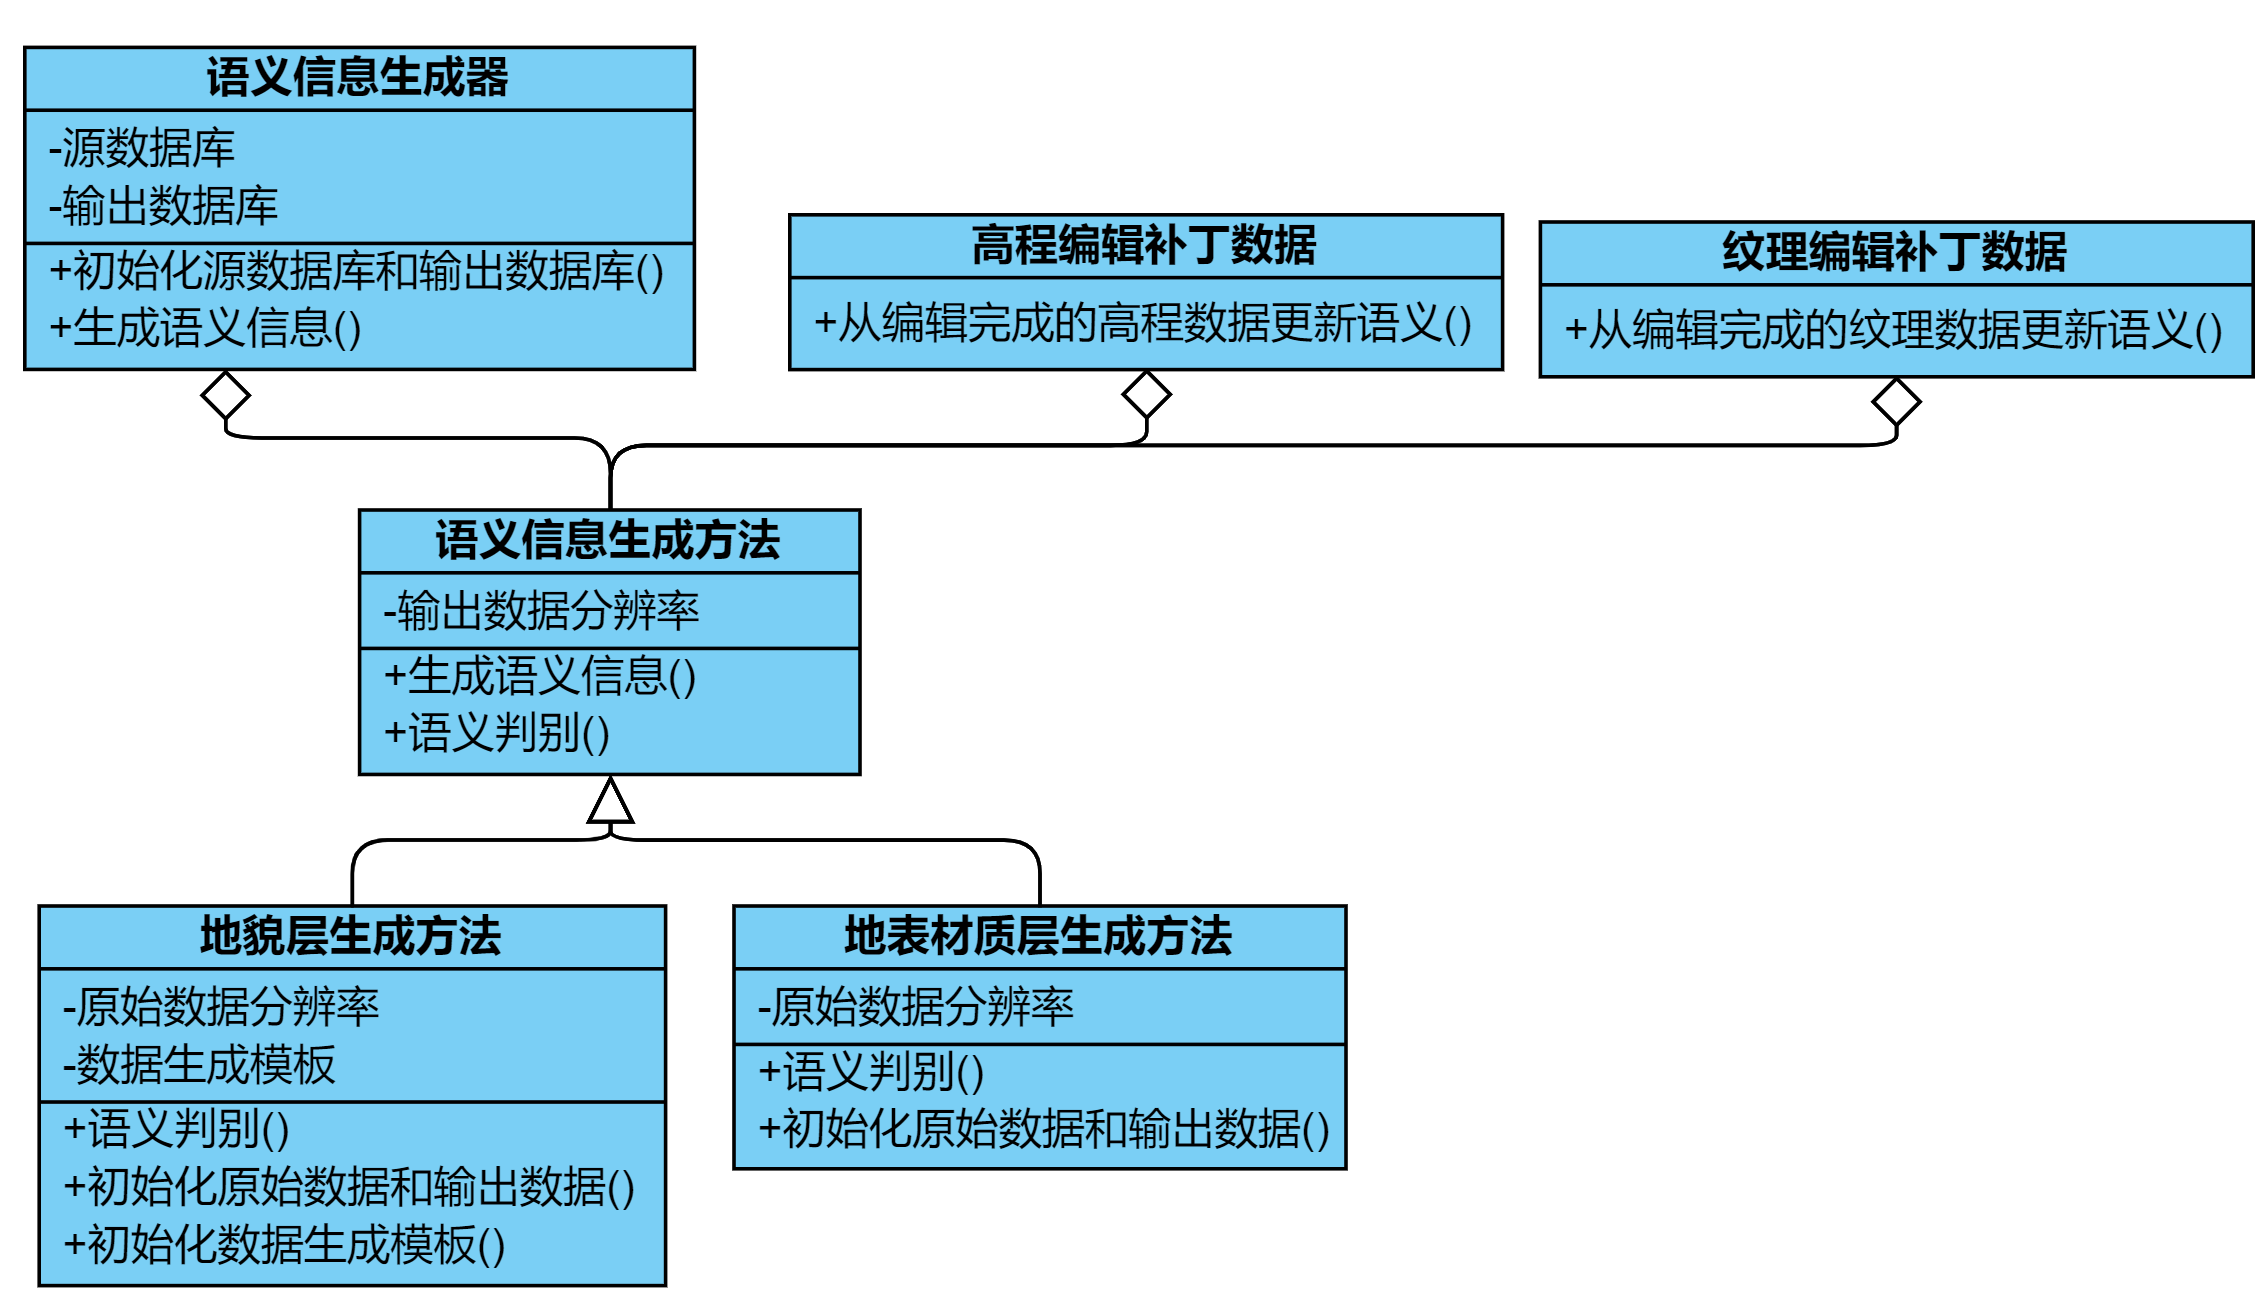
\includegraphics[height=5.6cm,width=9.3cm]{figures/semanticGen.png}
    \caption{语义生成模块主要框架}
\end{figure}
从高程和纹理数据生成的语义信息通常存在误差,需要手工进行修复,或进行更精确的定义。为了对语义信息进行手动编辑,首先需要将其可视化。预置一组颜色,以数组的方式进行存储,将语义信息以纹理的形式送入GPU后,在着色器中将语义信息映射为数组下标,为不同语义的地表叠加不同的颜色以进行区分。使用OpenGL纹理传递语义信息时需关闭纹理的线性滤波,避免出现错误的颜色过渡效果。\par
为了修复语义信息中的噪点和不平滑的边缘,笔刷是最直观的修复工具。语义信息的编辑与纹理信息的编辑可以使用相同的流程框架,但语义数据在获取数据和赋值上与纹理编辑有所不同。由于语义数据可能在块级别进行表示,因此如果对某个地形块进行笔刷编辑时首先为其分配像素级语义的内存,并用块语义进行填充。进行语义编辑时,具体的语义值相当于纹理编辑中的纹理材质,编辑时首先要选择要赋给语义信息的值。为语义信息赋值时,考虑到语义信息是非此即彼的,没有中间状态,因此对于笔刷权重值在[0.0,1.0]之间的笔刷模板,需要以某个中间值为阈值,笔刷权重高于阈值的,直接将该像素的语义赋值为目标值,否则不修改。\par
图6.3展示了从地形高程数据生成语义信息,通过手工编辑修复数据噪点,并将语义信息用于海洋模块绘制的工作流程。可以发现,使用语义信息指导的海洋模块绘制能产生更精细的海岸线效果,并更完整的保留码头等细长地形。图6.4展示了语义信息指导内陆水体绘制的效果。与使用纹理编辑工具产生的内陆水体效果不同,使用语义信息代替纹理蒙版信息来指导复合材质的绘制,可以只开启基础地形模块,而不加载地形编辑插件,更适应浏览阶段的需要。\par
\newpage
\begin{figure}[H]
    \centering
    \subcaptionbox{}{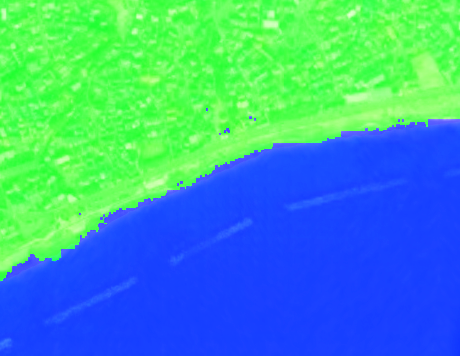
\includegraphics[height=4cm,width=6.5cm]{figures/semanticL.PNG}}
    \subcaptionbox{}{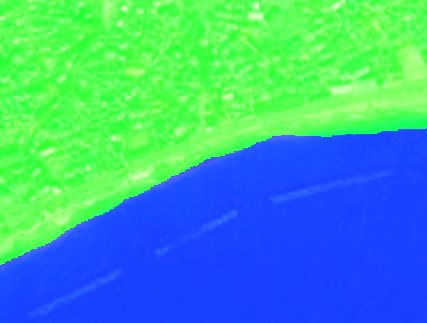
\includegraphics[height=4cm,width=6.5cm]{figures/semanticLA.PNG}} \\
    \subcaptionbox{}{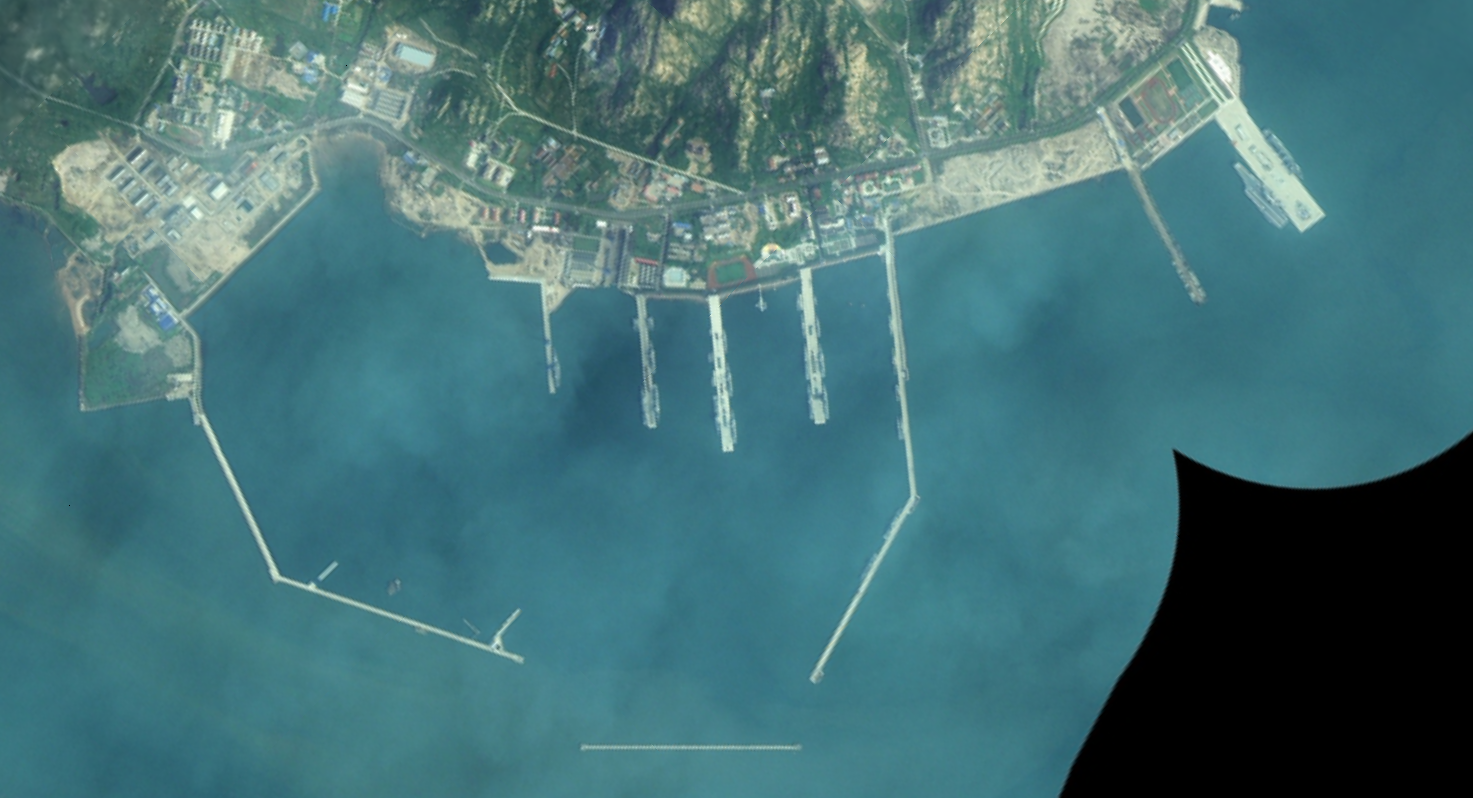
\includegraphics[height=4cm,width=6.5cm]{figures/shoreOri2.png}}
    \subcaptionbox{}{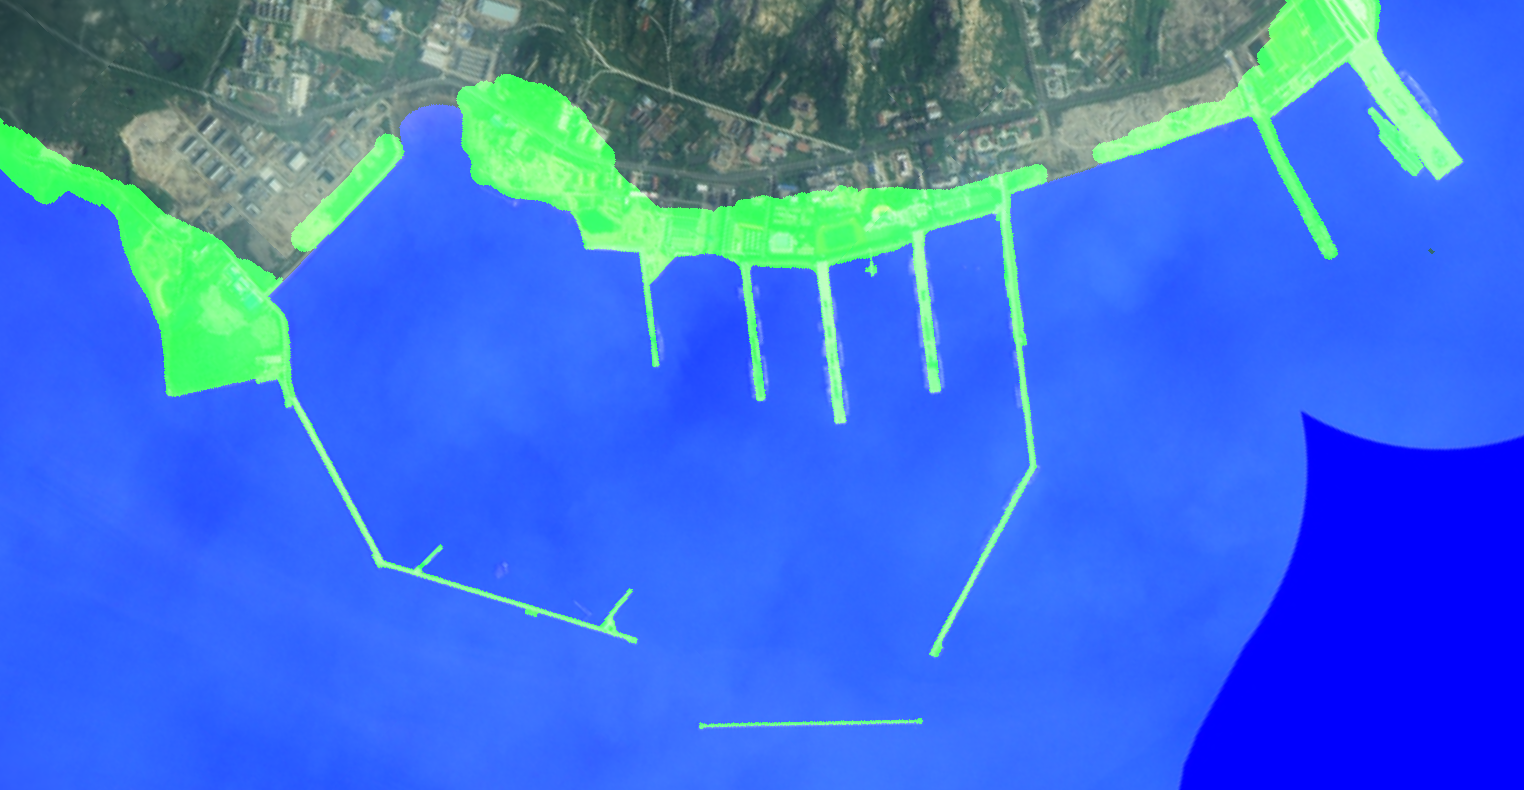
\includegraphics[height=4cm,width=6.5cm]{figures/shoreMask.png}} \\
    \subcaptionbox{}{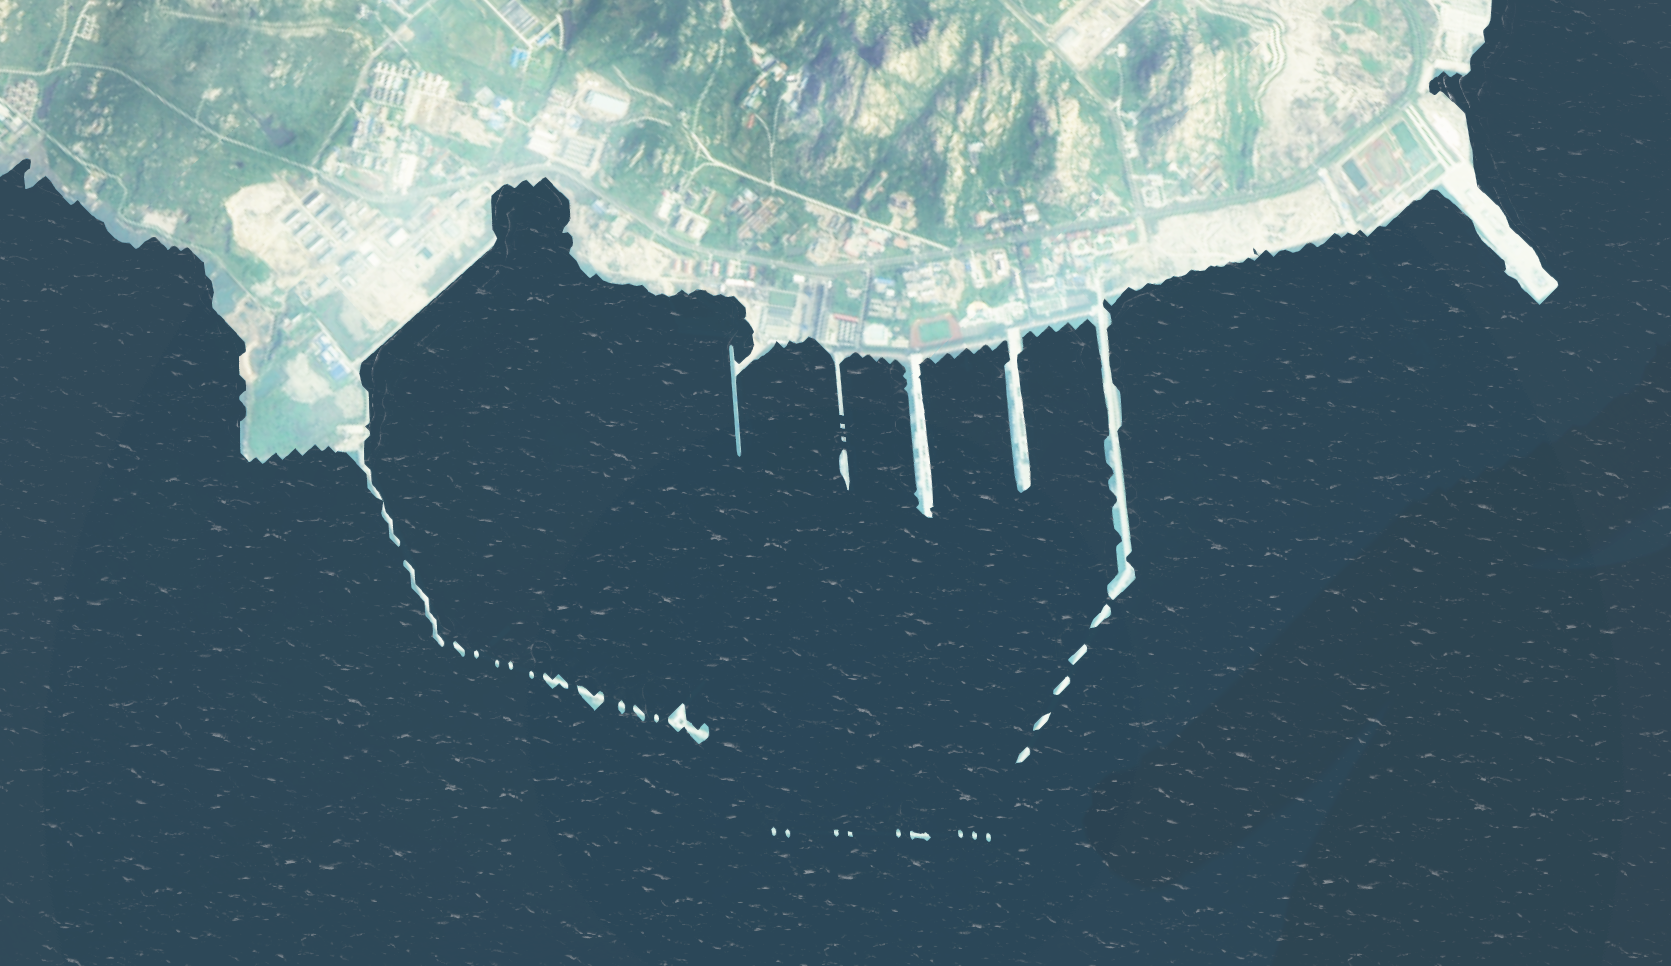
\includegraphics[height=4cm,width=6.5cm]{figures/shoreCompare.png}}
    \subcaptionbox{}{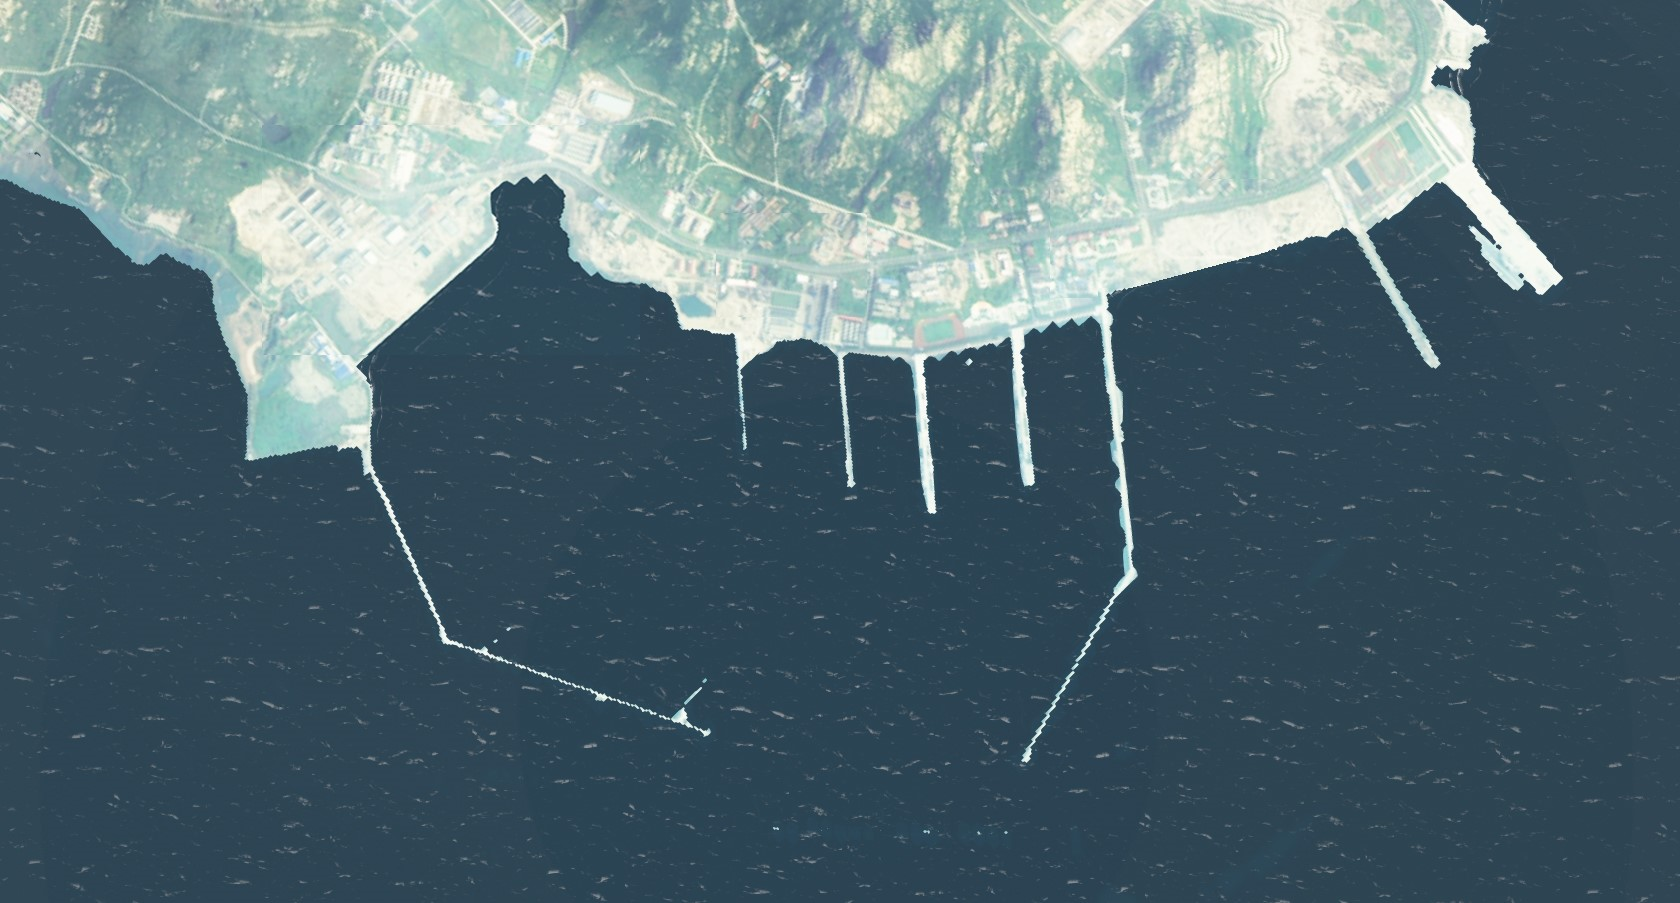
\includegraphics[height=4cm,width=6.5cm]{figures/shoreline.jpg}} \\
    \caption{海洋模块使用语义辅助绘制:(a).算法生成的海岸线不平整,噪点多(b).编辑后海岸线光滑,适用于海洋模块绘制海岸线(c).原始卫星影像(d).语义信息编辑结果(e).不使用语义指导的海洋绘制:较细的地形特征在高空视角中不能准确保留(f).使用语义指导的海洋绘制:可以在高空视角中保留码头等精细地形}
\end{figure}

\begin{figure}[H]
    \centering
    \subcaptionbox{}{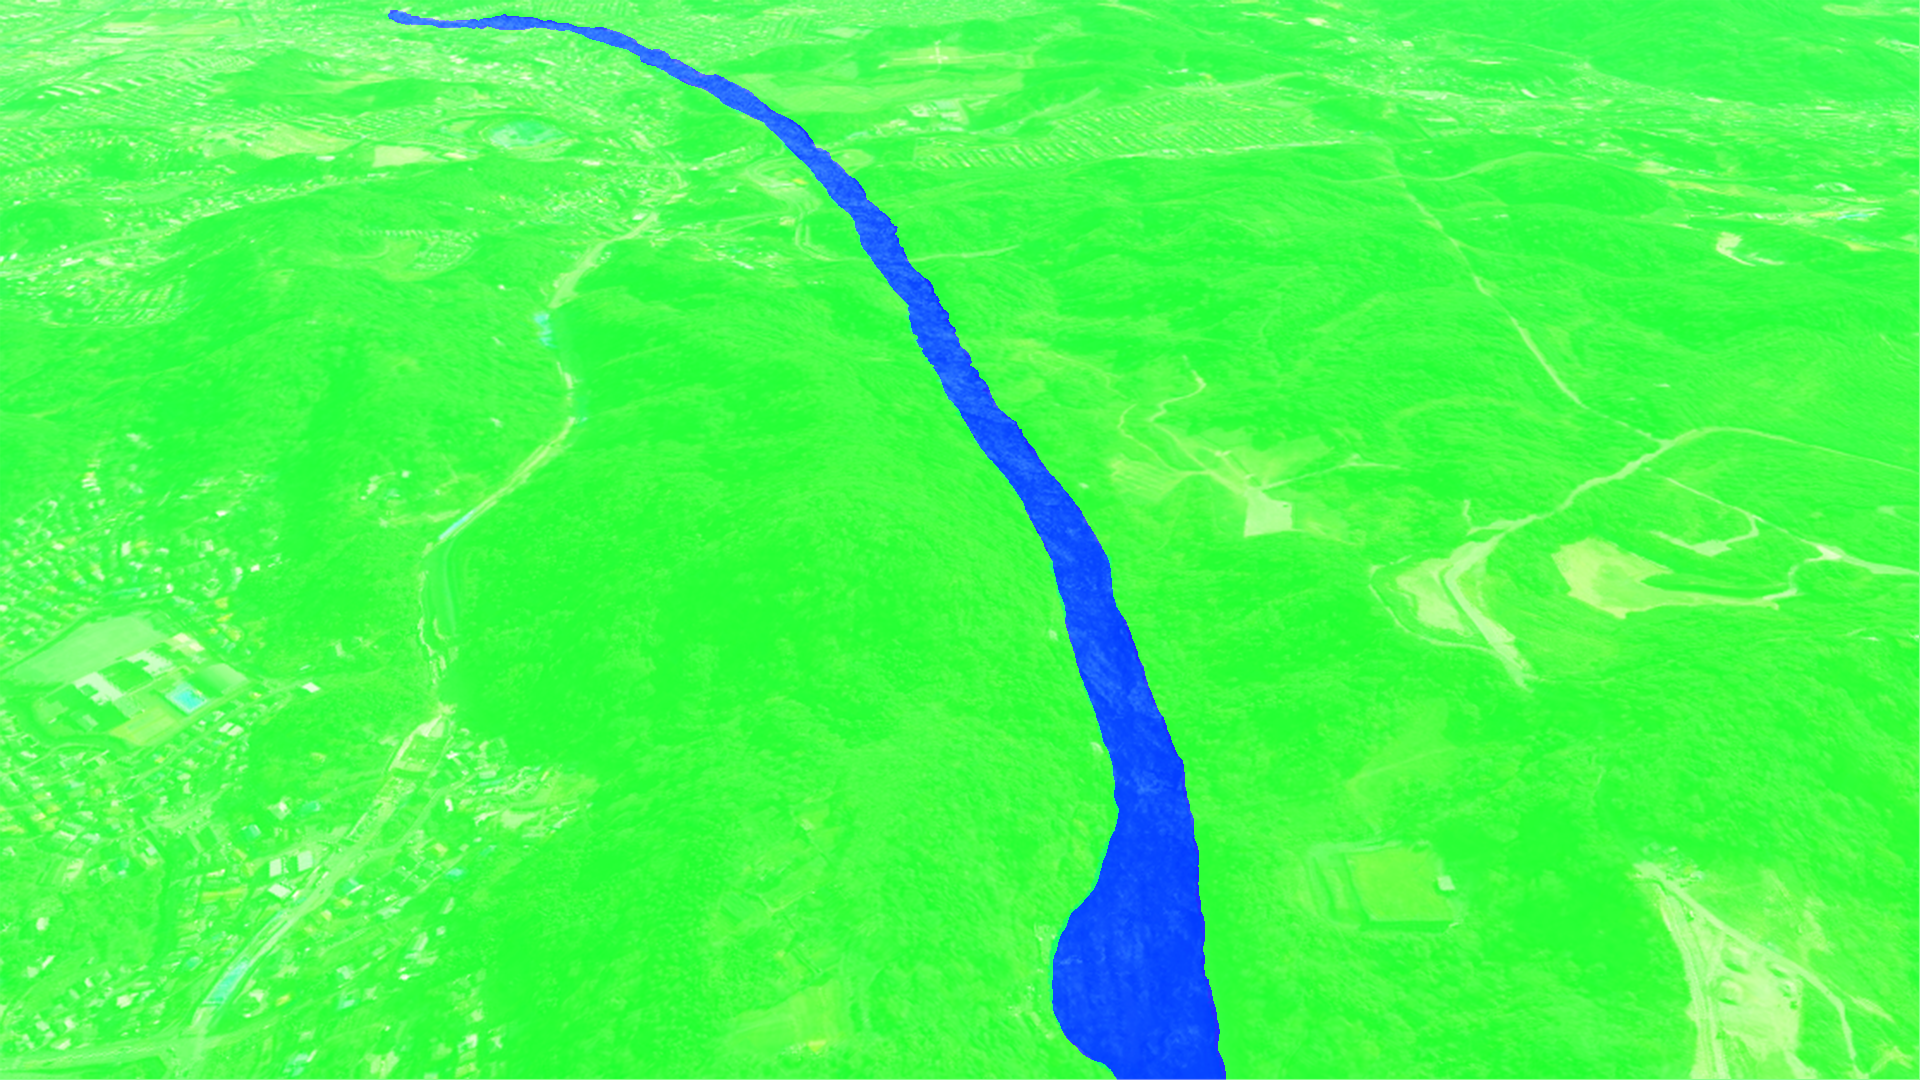
\includegraphics[height=4cm,width=6.5cm]{figures/riverNewSem.png}}
   \subcaptionbox{}{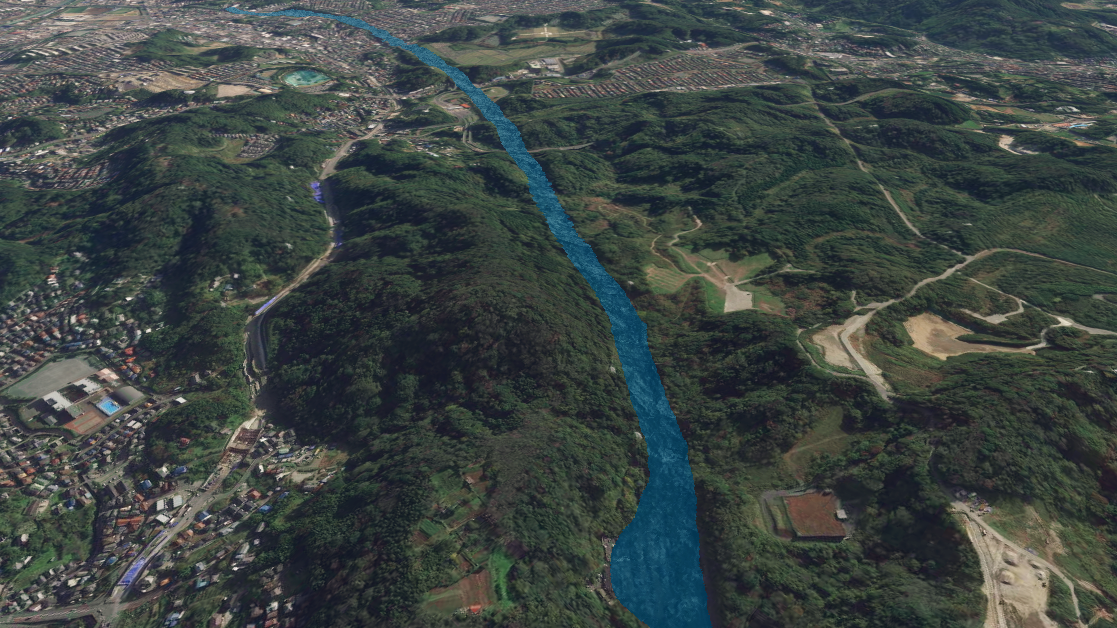
\includegraphics[height=4cm,width=6.5cm]{figures/riverNew.png}}
    \\
    \caption{依据语义信息产生的内陆水体效果:(a).语义信息,其中绿色表示草地语义,蓝色表示水体语义(b).内陆水体效果}
\end{figure}

由于语义数据会成为其他模块算法的输入,因此在对纹理和高程进行编辑的时候可能会相应的对地形语义造成影响,语义层需要根据新的纹理和高程数据进行更新。基于图6.2所示的框架,高程和纹理补丁数据可以在编辑结束时,构造一个编辑范围相同的语义补丁数据,将本次编辑生成的数据和初始化好的语义补丁数据传给语义生成方法。为了避免直接对整个地形块进行语义生成,覆盖其他语义编辑结果,可有选择的传入蒙版数据,依据蒙版只对特定下标的语义信息进行赋值。\par
图6.5展示了在高程-语义联动编辑状态下,进行高程编辑时,地形地貌语义层随高程变化而实时变化的效果。
\begin{figure}[H]
    \centering
   \subcaptionbox{}{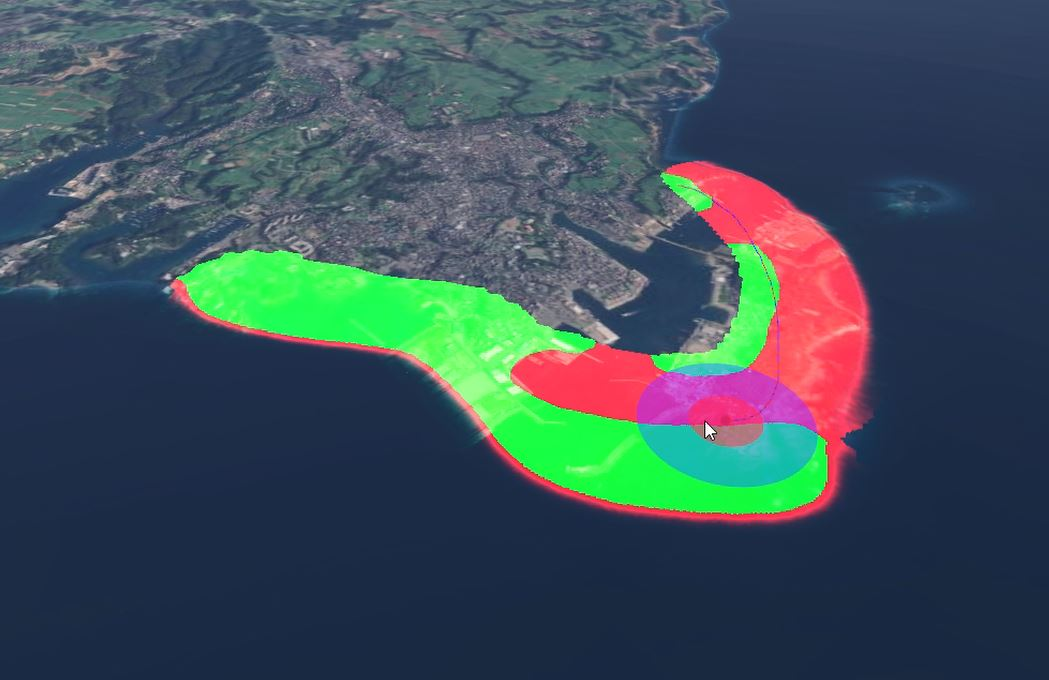
\includegraphics[height=3.7cm,width=6cm]{figures/linkageEdit.JPG}}
   \subcaptionbox{}{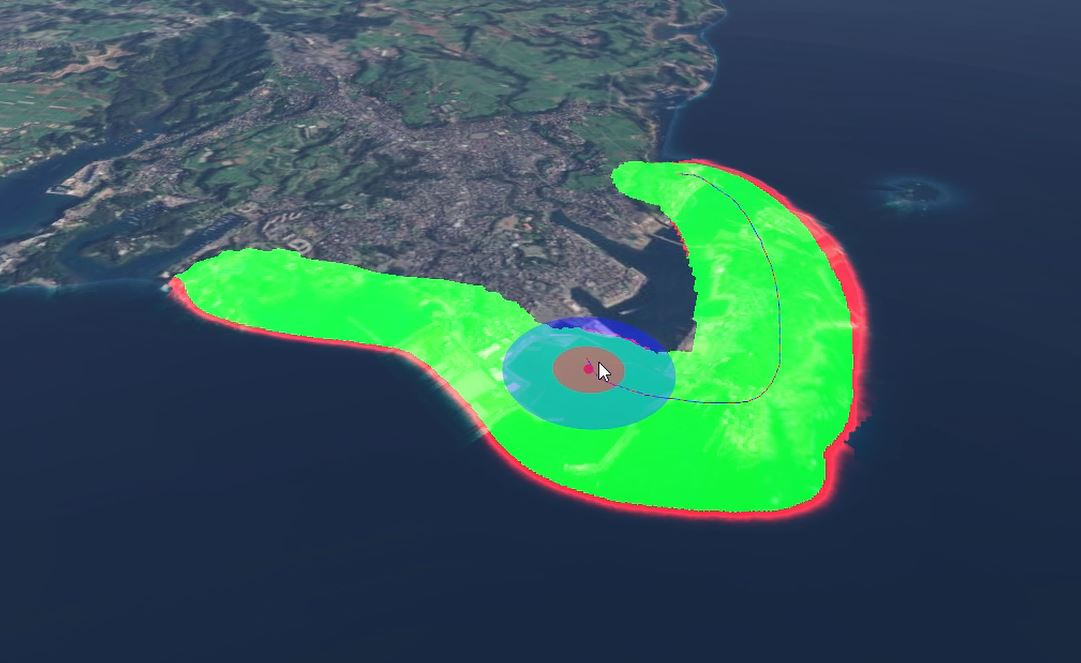
\includegraphics[height=3.7cm,width=6cm]{figures/linkage2.jpg}}
    \caption{高程-语义联动编辑效果:(a).高程编辑前(b).高程编辑后,语义信息发生变化}
\end{figure}
% vim:ts=4:sw=4

\section{本章小结}
本章首先介绍了语义信息的使用场景和研究意义,并对语义信息的定义进行了讨论。随后介绍了语义信息的生成方法和编辑方法,为了使语义数据与高程数据正确对应,提出了一种高程-语义联动编辑的方法,进行高程编辑时可以同时对语义数据进行更新。最后给出了使用语义信息指导海洋和内陆水体绘制的实例。